\documentclass{article}
\usepackage{graphicx} % Required for inserting images

\title{Assignment 3}
\author{Natalie Faraj }
\date{May 9 2023}

\begin{document}

\maketitle

\section{Introduction}
This assignment served as a thorough introduction to dealing with complex numbers on python, plotting and graphing various equations, aswell as experimenting with LaTex. Although tough, now that I have finished all my code, I feel as though I have learned many things. I now know more commands, techniques, and mathematical equations. This gives me an overall better understanding in computational astrophysics.


\section{Question 1}
The toughest part of this question was just understanding what it was asking; I went to my notebook and drew sketches before I actually coded anything. This question involves a complex plane which holds real and imaginary numbers; although I have a strong background in mathematics, this concept is always pretty tough to grasp. Since this question heavily involves mandelbrot sets, I had to do some research and makes sense of the equation first.


Once I figured out what I needed to do, I got to work. I imported all the modules I needed, I set boundaries (max/min values), set up the iteration, and plotted 2 images. Figure a shows a scatter plot where points that diverge are shown in gray dots (mostly scattered around the center). Figure b shows a similar depiction, except a colour scale indicates the iteration number at which the points diverge. These two figures are shown on the next page; notice the similarity in shape.

\begin{wrapfigure}{}{\textwidth}
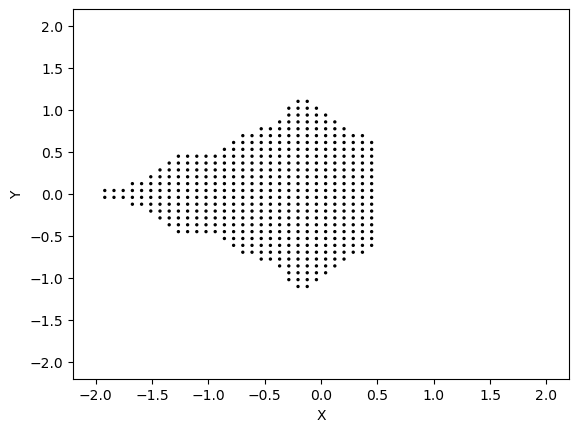
\includegraphics[width=0.5\linewidth,height=140\texthheight]{plot 1.png} 
\caption{Figure b}
\label{fig:wrapfig}
\end{wrapfigure}
\begin{wrapfigure}{}{\textwidth}
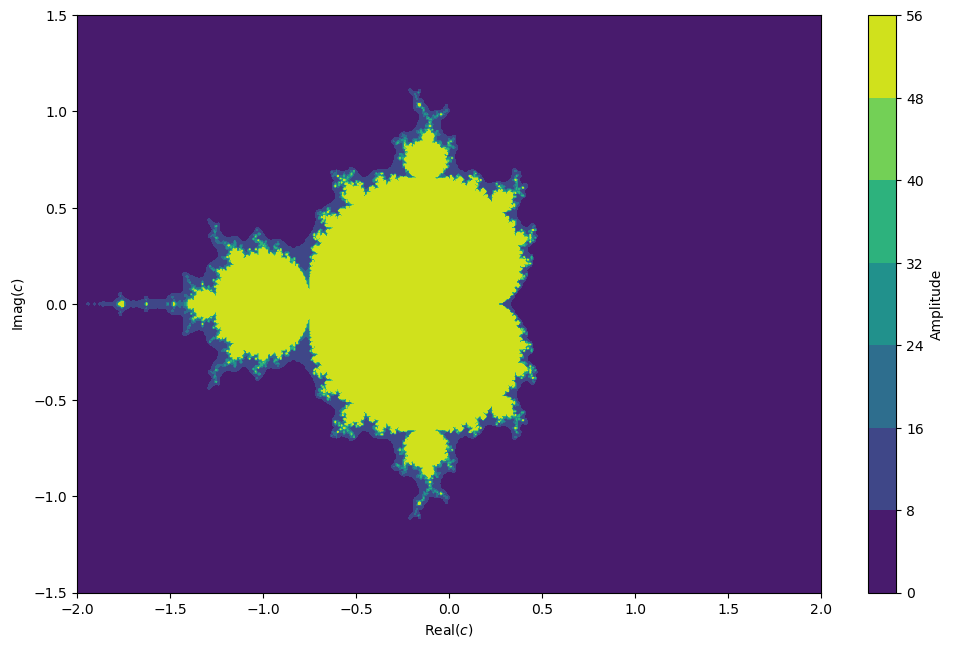
\includegraphics[width=0.5\linewidth,height=140\texthheight]{Colour scale.png} 

\caption{Figure a}
\label{fig:wrapfig}
\end{wrapfigure}

\section{Question 2}

Question 2 introduced a set of equations known as Lorenz' equations. These were derivatives that needed integrating. Firstly, I coded and defined the equations. Next, I used solveivp to actually integrate these set of equations. Then, we were told to recreate some plots of the Lorenz equations.
Figure 1 was composed of waves (keep in mind it's rotated here).

\begin{wrapfigure}{}{\textwidth}

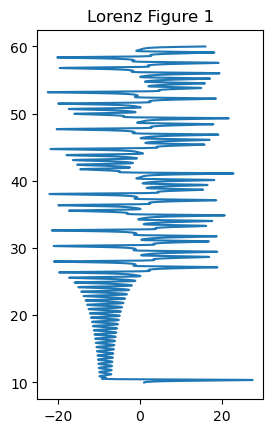
\includegraphics[width=.6\linewidth,height=280\texthheight]{Lorenz_figure_1_rotated.png} 
\caption{Figure 1}
\label{fig:wrapfig}
\end{wrapfigure}

Figure 2 was composed of two 2D graphs; these were X vs Y (in yellow below) and Y vs Z (in green below).

\begin{wrapfigure}{}{\textwidth}

\includegraphics[width=1\linewidth,height=160\texthheight]{Lorenz_other_figure_2.png} 
\caption{Figure 2}
\label{fig:wrapfig}
\end{wrapfigure}

Then, I wanted to experiment with some 3D graphing, thus I plotted the 3D Lorenz plot (figure 3, shown below):

\begin{wrapfigure}{}{\textwidth}

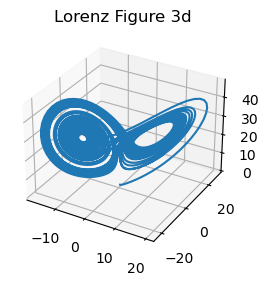
\includegraphics[width=.6\linewidth,height=280\texthheight]{Lorenz_3d.png} 
\caption{Figure 3}
\label{fig:wrapfig}
\end{wrapfigure}

Lastly, I conjured up a series of commands that allowed me to find the distance between W and W'.
Then I was able to graph this on a semilog. It can be seen on the next page (Figure 4)
\begin{wrapfigure}{}{\textwidth}

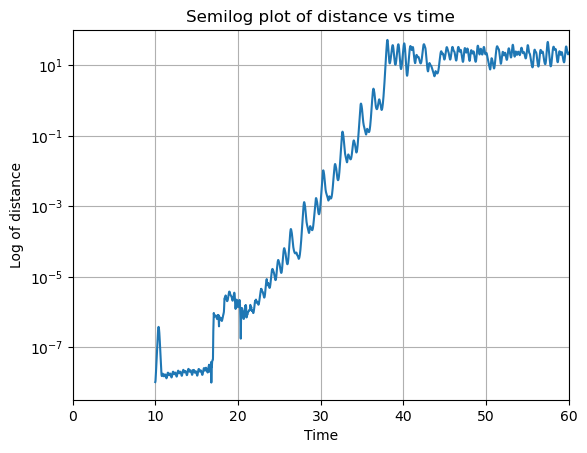
\includegraphics[width=.6\linewidth,height=280\texthheight]{Semilog.png} 
\caption{Figure 4}
\label{fig:wrapfig}
\end{wrapfigure}

\section{Conclusion}
In conclusion, I learned a lot from this assignment. I plotted new equations, learned new commands, and picked cool colours for Lorenz' equations!
I also can't forget to mention that I also learned to use LaTex (case in point).

\end{document}